\documentclass[letter:wpaper]{article}
\usepackage{isea}
% UPDATE: See the local /.vscode/settings.json
% The pdftex option is necessary for the pdfinfo command to work, for the graphicx package to work, and for the correct fonts to work. It requires the pdfLaTeX renderer
% [1] Select the Preferences: Open User Settings (JSON) command in the Command Palette (⇧⌘P)
% [2] Find the latex-workshop.latex.recipes setting and move the "xelatexmk" recipe to the top of the list. This will make xelatexmk the default recipe for building LaTeX files.
%
%   "latex-workshop.latex.recipes": [
%     {
%       "name": "latexmk",
%       "tools": ["latexmk"]
%     },
%     {
%       "name": "latexmk (xelatex)",
%       "tools": ["xelatexmk"]
%     }
% [3] There is no 3. There is already a "latex-workshop.latex.tools" setting for "latexmk" that uses the -pdf flag and so will use pdfLaTeX. I suppose [3] is for putting xelatexmk back as the default recipe
\usepackage[pdftex]{graphicx}
\pdfinfo{
    /Title (Art as Technology)
    /Author (Kynan Stewart Hughes)
}
\usepackage{times}
\usepackage{helvet}
\usepackage{courier}
\usepackage[numbers]{natbib}
% The file isea.sty is the style file for ISEA 2025 proceedings.
%
\title{Art as Technology (v1.1.0.5)}
\author{Kynan Stewart Hughes\\
Creativity and Cognition Studios\\
University of Technology Sydney\\
Sydney, Australia\\
kynan.s.hughes@student.uts.edu.au\\
\newline
\newline
}
\setcounter{secnumdepth}{0}

\begin{document} 
% Setting the default tolerance level
% \tolerance=200
% Setting a high tolerance level
% \tolerance=10000
% Some more drastic measures for hbox issues
% \emergencystretch=4em
% \raggedright
\maketitle
\begin{abstract}
    This paper argues that art should be understood as a form of technology: a system programmed for affective and conceptual purposes. Drawing on complexity science and Process philosophy, it frames art as a codifying practice that reconfigures materials and meanings to produce emergent effects. Rethinking art in technological terms also invites a broader, more ethically attuned understanding of technology itself. The author’s own artwork contributes to this argument. The paper concludes by encouraging artists working with emerging technologies to embrace a mode of crafting grounded in interdependence, emergence, and ethical responsiveness.
\end{abstract}

\keywords{Keywords}

Art, technology, complexity, aesthetics, affect, information, craft, ethics, systems, emergence, meaning, constraints, coarse–graining

\section{Introduction}

    This paper explores the idea that art is a technology \citep[pp.74–75]{SauvagnarguesArtmchns2016} \citep{GellThTchnlgyOfEnchntmnt1992} \citep[p.202]{OSullivanFrmAsthtcsToThAbstrctMchn2010}. It is an idea that grounds art as a material practice and makes technology make a different kind of sense as a field of practice that includes artmaking. 
    
\section{A Definition of Technology} 

    A technical object is always ``a phenomenon captured and put to use.'' \citep[p.53]{theNatureOfTechnology2009}. To put it another way, technology is ``programming [...] phenomena for [...] purpose.'' \citep[p.53]{theNatureOfTechnology2009}. This distillation holds for all technologies, contemporary and historical. ``Phenomena'' don't have to be physical, like fire or electricity. They may be ``behavioural or organisational  effects'' \citep[p.55]{theNatureOfTechnology2009}, or ``truism[s] of nature'' \citep[p.45]{theNatureOfTechnology2009}.

    \subsection{Example: Money}

    For example, Money is a technology.

    \begin{quote}
        The monetary system makes use of the ``phenomenon'' that we trust a medium has value as long as we believe that others trust it has value and we believe this trust will continue in the future. \citep[p.55]{theNatureOfTechnology2009}
    \end{quote}

\section{A Definition of Art}

    Jacques Rancière has called contemporary Western art the \emph{aesthetic regime}. It is not a single coherent paradigm, but a plurality of ``frequently different, and sometimes contradictory, ways of thinking'' \citep[p.8]{RanciereMdrnTms2022} organised around the idea of aesthetic experience. It's emergence at the end of the eighteenth century coincided with Emanuel Kant's \emph{Critique of Judgement} \citep[pp.23–24]{RancierPltcsOfThAsthtcs2004}. 

    Within this regime, all distinctions and differences operate in relation with the idea of aesthetic experience. Styles like Modernism and Post–Modernism, for example, are simply different strategies for making aesthetic objects within the aesthetic regime \citep[p213]{ZepkeSblmArt2017}. Art which is anti–aesthetic is operating within the aesthetic regime by being self–consciously critical of it\footnote{
        Reference.
    }. Conceptual art is art that invites us to consider the aesthetic potential of ideas\footnote{
        Reference.
    }.

    Art in this sense is a complex codifying system that dislocates objects from their original functions and meanings and gives them new functions and meanings. The ``dissensual operation'' of creating an artwork, for example by working a material into a form, or by setting the state of pixels on a screen, or by appropriating a ready–made object, literally ``transforms a given form or body into a new one.'' \citep[p.54]{RancierThEmncptdSpcttr2009}.

\section{Affect}

    The concept of \emph{affect} \citep{MassumiTheAtnmyOfAffct1995}, is a way of thinking about how things affect other things in the complex interconnected systems of material reality. Affect is a kind of intensive, interactive event. It is human and inhuman, organic and inorganic.

    Affect is when emergence happens. It is a quantum shift ``fed forward'' across progressively higher levels of reality \citep[p.37]{MassumiPrblsFrThVrtl2002} until it may register on human perception as apparent cause and effect. According to the science of complex systems, this apparent causality echoes back as ``downward causation'' \citep[p.?]{FlackCrsGrnng2017} that constrains and influences the behaviour of system components, so that affective exchanges are happening all the time at all levels of organisation.
    
    Humans are particularly good at attributing affective regularity to objects \citep{FristonThFrEnrgPrncpl2010} \citep{DeaconTheSymbolicSpecies1998}. We notice patterns: regular cycles of seasons and plants, behaviours of animals, the organisation of sounds into music and languages.
    
    Art, the aesthetic regime, is system of codes that exploits our capacity for noticing affective regularity. It is a hack on our capacity for attributing affective power to objects. Through a process of becoming art, an object is packed with affect, like a battery holding a charge. 
    
    The affective charge of an art object can consist of any combination of qualities – strong, weak, sensorial, semantic, abstract, pleasant and unpleasant et cetera. It can be a sense of the beautiful, or it can involve concepts and feelings that are more difficult to pin down. It can, like a Patricia Piccinini sculpture, strobe between incompatible affective states, such as the cute and the grotesque. Like a readymade, it can call attention to the codifying power of art itself.

    The relatively recent move equating aesthetic experience with affect is a shift away from the idea that some normative experiences are better than others (beauty), and towards the messy reality of material processes. It contextualises aesthetic experience in a complex ecology of affect. Art is now about “complex affective and intensive exchanges, situated in the broader ecology of the world.” \citep[p.155]{HighmoreBttrAftrTst2010}

    \section{Purpose}

    According to Felix Guattari, art ``confers a function of sense and alterity to a subset of the perceived world.'' \citep[p.131]{GuattariChsmss1995}. In other words, the point of an artwork is to be \emph{about} something.
    
    Arthur Danto said that artworks are ``embodied meaning'' \citep[p.125]{DantoEmbdMnngs2007}, and meaning is a useful way to think about the affective purpose of art objects as long it is remembered that an art object's meaning is always contextual\footnote{
        Manuel DeLanda has pointed out that the words ``meaning'' in the expressions ``this word has a meaning'' and ``this life has a meaning'' are two entirely different words'' \citep[pp.40–41]{DeLandaCsltyAndMnng2018}. Suggesting, as for example Noël Carroll has, that Danto's idea of embodied meaning is too narrow, is to assume the first sense of the word meaning, which is the simple signifier/signified sense.
    }. ``Meaning is [...] a network of enveloped material processes. A thing has as many meanings as there are forces capable of seizing it.’'' \citep[p.10]{MassumiAUsrsGdTCptlsmAndSchzphrn1992}.

    However, the question of purpose is not easily left at that because it has traditionally been used to differentiate artmaking from other crafts. For Kant, art objects, which for him meant beautiful objects, were necessarily ``purposive without a purpose'' \citep[p.57]{KantCrtqOfJdgmnt}. The very essence of an artwork was seen to be its lack of functional purpose (as if being art was not a functional purpose).
    
    This is a weirdly circular and weirdly enduring idea, and it has been the bases for other weird ideas such as the idea that art objects are ``autonomous''\footnote{
        Reference: Greenberg
    }. It only makes sense if one is already looking for a reason why art is different to other kinds of making and doing, which of course Kant was.
    
    It also depends on an assumption that objects are fixed, independent things with fixed, independent purposes. Over the last eighty year or so, an awareness of the ubiquity of complexity has emerged in Modern Western thought, and it is now possible even for those of us living in Modern Westernised cultures to see that all objects, along with their purposes and meanings, are entirely dependant on context.

    For example, as well has having embodied meaning, which might be termed their ‘art purpose’, art objects always also have other, ‘non–art’ purposes. While the art purpose of a painting may simply be to evoke an experience of beauty, at the same time it may confer status, be an investment, or start a revolution. If art objects have as many meanings as there are forces capable of capturing them \citep[p.4]{DeleuzeNtschAndPhlsphy2006}, then the same thing can be said of their non–art purposes.

    The affective charge of an art object may derive, to some extent, from a non–art purpose, but is never reducible to it. There is always ``contextual excess or remainder'' \citep[p.252]{MassumiPrblsFrThVrtl2002}.
    
    When art purpose and non–art purpose become confused in an artwork, it is the art purpose that suffers. This is particularly relevant for artists who work with emerging technologies because the non–art purposes of emerging technologies are exciting and not fully understood.
    
	In the early 2000s, practitioners of locative art were criticised for their uncritical use of mapping and networked, location-aware, mobile technologies, as well as for their collaborations with industry. It was alleged that they lacked a structure of accountability and ethics, were ushering in a `society of control', and were turning the media-art conference circuit into a `shopping-driven [...] spectacle' \citep[p.358]{beyondLocativeMedia2006}. Locative art was described as a ``technocentric fantasy'' that ``downplays [...] history'' \citep[para. 2]{questioningTheFrame2004}.
    
    The art purpose of locative art was being interfered with by the imagined non–art purposes and potentials inherent in applications of locative technologies. Today, as we grapple with the conjunction of rampant technology-fuelled capitalism and mass surveillance, these imaginings seem to have actualised. 

    Incorporating non–art purpose into the meaning of an art object is a risky strategy, which is what makes it interesting. In socially connected art, participatory art, and art that is made to be used (craft and design), for example, non–art purpose and art purpose are productively entangled. 
    
    Should the meaning of an art object become reducible, for the viewer, to a non–art purpose, it would have ceased to be an art object.

    \subsubsection{Example: \emph{FlowAttractor}}

    \begin{figure}[h]
        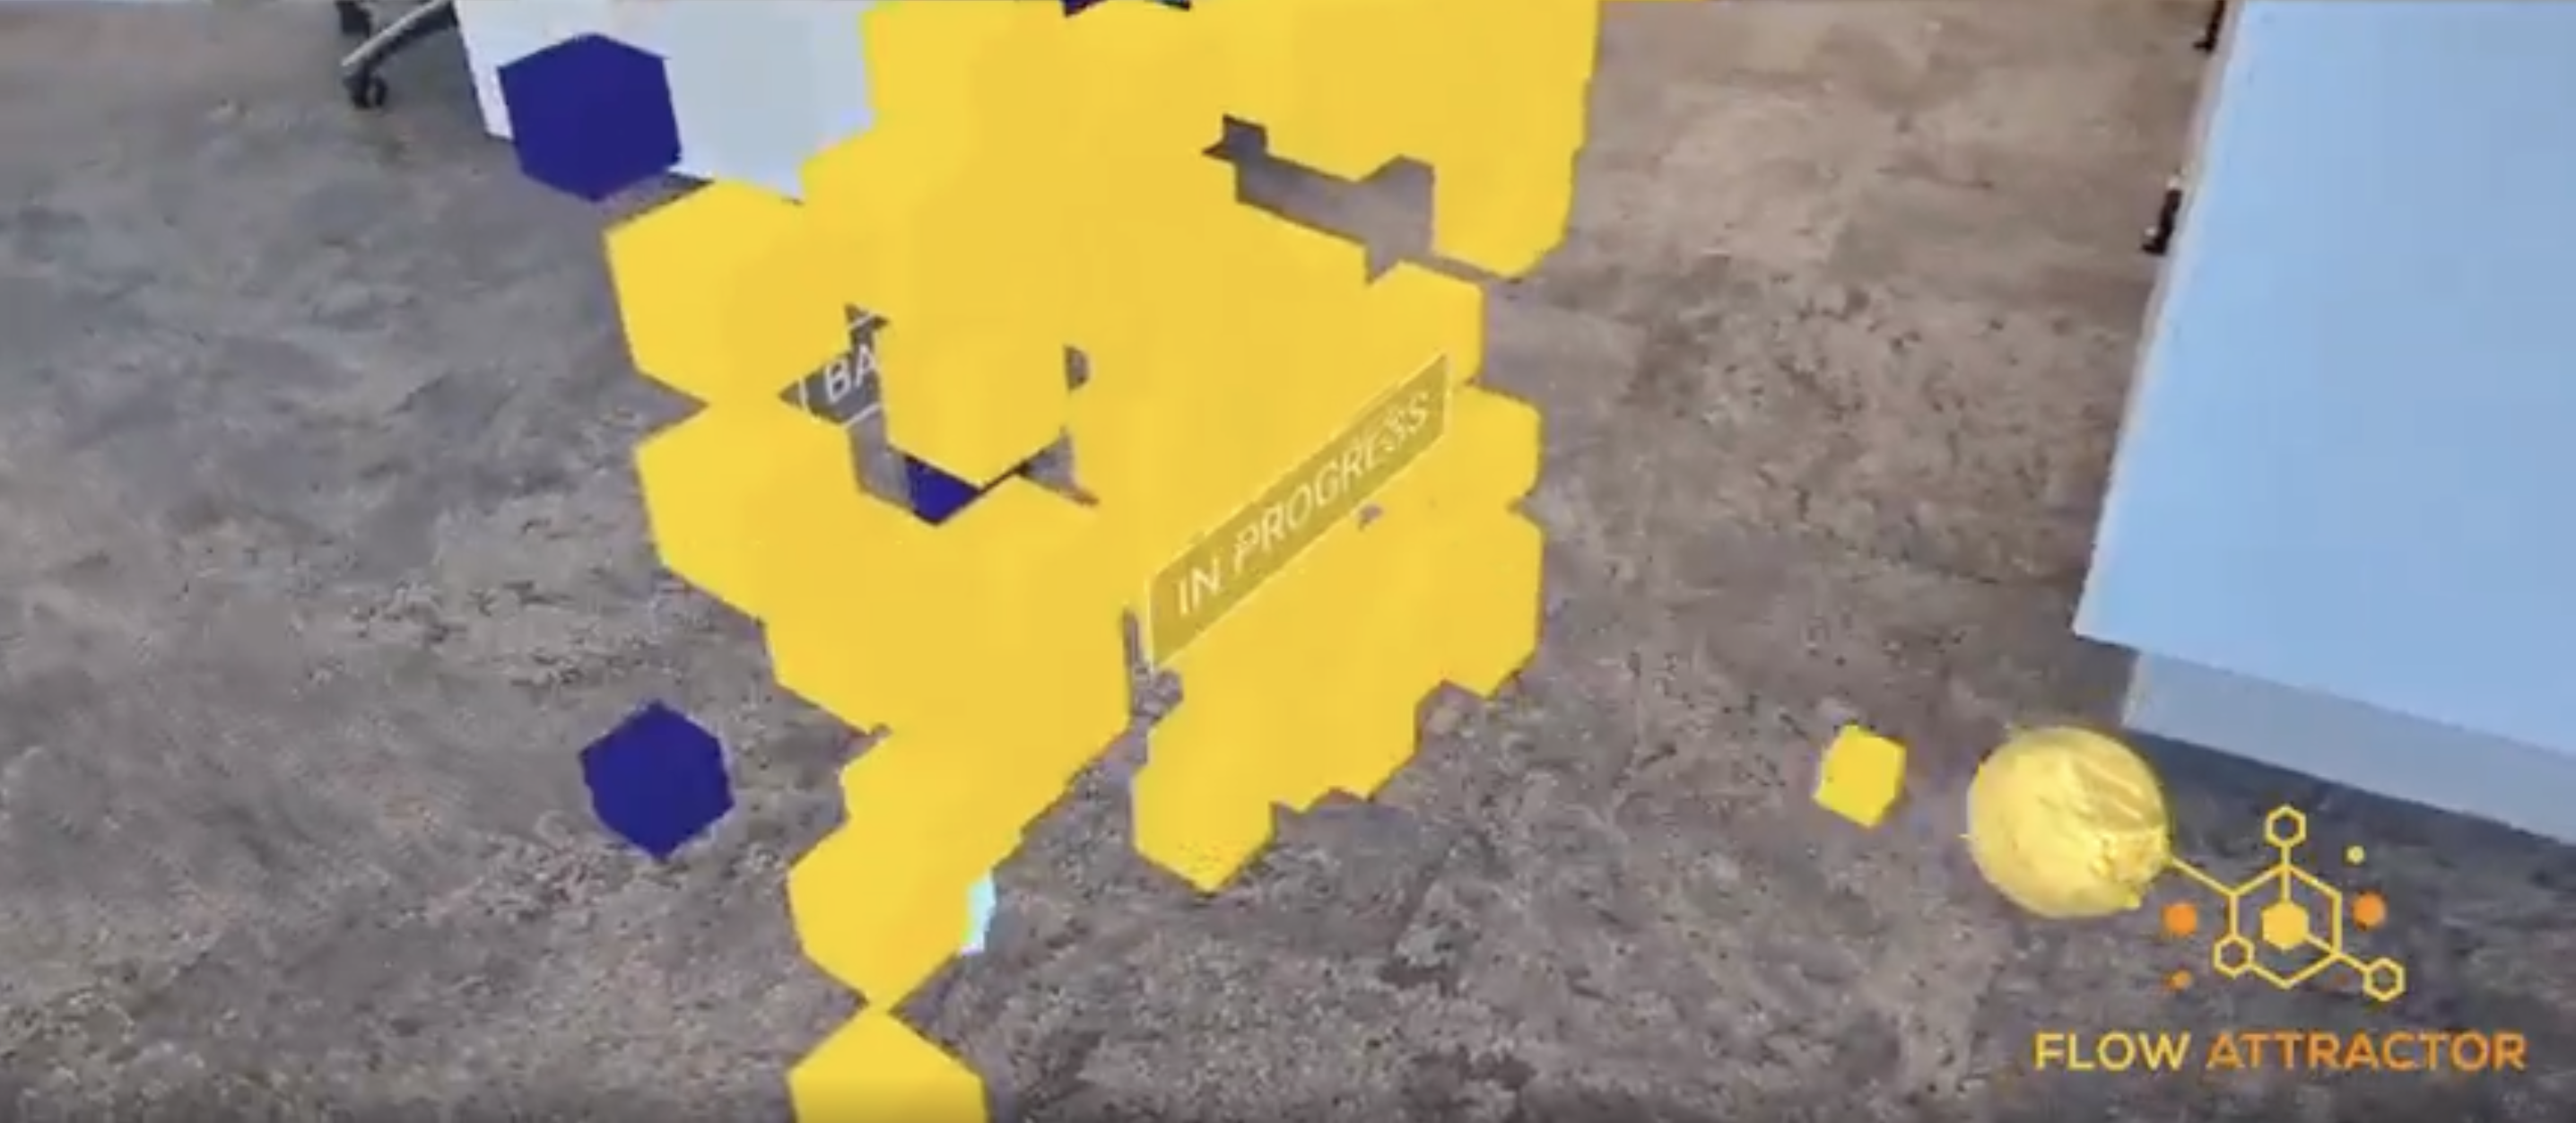
\includegraphics[width=3.31in]{flow-attractor.png}
        \caption{\emph{FlowAttractor} models complex workflows as flying cubes. \copyright Respect Copyright.}
        \label{fig:flow-attractor}
    \end{figure}

    In \emph{FlowAttractor} (Figure~\ref{fig:flow-attractor}), the flow of the blocks represents the otherwise invisible flow of work items through the software production system of a bank. The piece is an experiment to find out what can happen when an art object is integrated into a business context. Its non-art purpose within the organisation is to catalyse an awareness of the effects of making small decisions designed to improve the flow of work through the system. It works surprisingly well in this way. However, because its purpose is, in that context, ultimately reducible to a non–art purpose, it is effectively not art.
    
    Of course, if we allow that an art object's purpose is ``multidimensional'', ``contextually complex and indeterminate'' \citep[p.25]{HoelscherThPtcsOfPhsSpc2014}, then we must attribute the same complexity and indeterminacy to [other] technical objects. This is actually very easy because examples abound. We don't know precisely why anaesthesia works\footnote{
        % Reference: Franks, N.P. (2006). “Molecular targets underlying general anaesthesia.” British Journal of Pharmacology, 147(S1), S72–S81. Franks notes that although many targets have been proposed (e.g. GABA_A receptors), there is no single unified theory of how anaesthetics produce unconsciousness.

        % “Despite more than 150 years of use, the precise mechanisms by which general anesthetics induce unconsciousness remain elusive.” ~ Brown et al. (2010), The New England Journal of Medicine, 362(9), pp. 856–865.
    }. Viagra was a treatment for angina\footnote{
        % Reference: Boolell, M. et al. (1996). “Sildenafil: an orally active type 5 cyclic GMP-specific phosphodiesterase inhibitor for the treatment of penile erectile dysfunction.” International Journal of Impotence Research, 8(2), 47–52.
    }. Microwave ovens were developed because a radar technician's chocolate bar melted in his pocket\footnote{
        % Smithsonian Magazine, “How the Microwave Was Invented by Accident” (2016) and Klooster, J.W. (2009). Icons of Invention: The Makers of the Modern World from Gutenberg to Gates. ABC-CLIO.
    }. The internet is a military communications system for sharing AI generated shrimp Jesus videos, and for enabling mass surveillance. 

\section{A Fold in the Distribution of the Sensible}
    
    According to science, a phenomenon called ``coarse graining'' occurs when a subsystem with apparently emergent properties is treated as a single entity for predictive purposes by components of a complex system. Coarse graining works by ignoring the details. When it works, it is an efficient, ``lossy but true'' \citep[p.4]{FlackCrsGrnng2017} strategy.

    Sometimes, however, it is just lossy \citep[p.8]{FlackCrsGrnng2017}. People have been hard–wired by evolution to see patterns, to the extent that we tend to imagine them \citep{FristonThFrEnrgPrncpl2010}.
    
    It seems likely that this has been the case with the perceived pattern of difference that separates art and technology. The split between art and other kinds of making is, I suggest, a dodgy piece of coarse graining that has been with us for about six hundred years. This is possible because the aesthetic regime is overlaid upon an older regime that laid the foundations for it. 
    
    \subsubsection{The Regime of Representation}

    The idea of there being a qualitative difference between the practices we now call ‘the arts‘ and other ways of doing and making began taking shape during the Renaissance \citep[p.136]{TatarkiewiczWhtIsArt1971}. By the 17th century the classification of various practices as ``the arts'' had become firmly established. Rancière has called this \emph{partitioning of the sensible} the ``regime of representation''\footnote{
        Reference.
    }.
    
    Although the various \emph{arts} existed – understood as forms of knowledge and their applications – they were not recognised as part of a singular, overarching category of human experience called ``art''. The arts – music, literature, sculpture, painting, et cetera – were disparate practices serving different social functions, and were situated within a stratified system that categorised activities and the individuals engaged in producing them. The job of the arts was to represent the world as a unity of sensible order. A place for everything and everything in its place, including people.
    
    The aesthetic regime -- art as we know it today -- is a tactic that cuts across the regime of representation, but we still observe the fold of difference that separates the arts from other ways of making. For example, we organise our our university faculties and school curriculums along it: science, technology, engineering and maths on one side, the arts and humanities on the other. 
    
    It is this fold in the ``distribution of the sensible'' \citep[p.42]{RancierPltcsOfThAsthtcs2004} that the idea of art as technology smooths out. What would it be like, one wonders, for this fold not to exist?  A look at the regime that proceeded the regime of representation reveals a situation in which the fold did not exist.
    
    \subsection{The Ethical Regime of Images}

    Heidegger, in his essay ``The question concerning technology'', pointed out that ``techne'' was the ancient Greeks' word for skill, craft, and technique. The term covered ‘the arts’ as well as sciences, and technical domains like sword-making and shipbuilding \citep[p34]{HeideggerThQstnCncrngTchnlgy1954}.
    
    Rancière has called the mode of thought that prevailed at this time the \emph{ethical regime of images}, the word ``image'' referring to the idea that all made things in the world are instances of ideal, universal forms.

    At this time, ethical concerns were primary. The ``end or purpose'' of crafted objects mattered a great deal: the uses they were put to, the effects they resulted in -- in general the way their modes of being affected the ``ethos'', ``the mode of being of individuals and communities'' \citep[pp.20–21]{RancierPltcsOfThAsthtcs2004}.

    Plato thought in terms of \emph{true arts}, which are forms of knowledge based on the imitation of a model with precise ends, and \emph{lesser arts} that simply imitate appearances \citep[p.20]{RancierPltcsOfThAsthtcs2004}. These ideas, which now seem quaint, were nonetheless an ethical framework informed by a concern for the connection between actions and their potential effects.

    Like the regime of representation, the ethical regime of images still operates as a kind of substrate. We care about who produces what and to what effect, especially when it comes to art.
    
    In Australia in 2021, an art festival in Hobart planned to include a piece by Santiago Sierra, which involved a call for donations of blood from descendants of First Nations peoples who survived the genocidal effects of Tasmanian colonisation. First nations people around Australia argued that the piece would emphasise the bloody aspects of colonization for no positive effect. Rappers Tasman Keith and Briggs commented on Instagram that they ``already gave enough blood" \citep{DrkMfBld2021}. The festival organisers eventually apologised and cancelled the piece.
    
    Somewhere along the line technological crafting became decoupled, in a way that artmaking didn't, from the kind of exquisite sensitivity to affect which is ethics. Technology evolves, it seems, regardless of how we feel about it. For example, while many people fear the potential effects of AI generated content, while we might fear losing our jobs or our signature styles to the proliferation of technological systems that can do what we do at a different economic scale, our feelings on these matters will be ignored.
    
\section{Conclusion: Thinking across the fold}

    To think of art as a technology is to think across the fold that separates art from technology, and to begin a process of smoothing out the fold. It challenges us to wonder what it would be like for this difference to not exist, potentially changing the way we think about both artmaking and technological development.
    
    If the difference between art and technology that causes it to be unthinkable to think of art as a technology can be rethought, then perhaps it is a job for artists who work with emerging technologies. 
    
    As artists working at the edges of technological evolution, we are invited to return humanity to an idea of crafting, guided by ethics informed by an appreciation of the complex, interconnected nature of all things. Perhaps we will open a space in which humans can begin to learn how to craft with our technologies differently at the very moment in history when our technologies are learning to relate differently with us.
    
    To paraphrase Gilbert Simondon, we may perhaps begin to think of ourselves as

    \begin{quote}
        inventors of technical and living objects. We coordinate and organise their mutual relation at the level of machines, between machines. [...] We construct the signification of the exchanges of information between machines. Our rapport with the technical object is a coupling between the living and the non–living. \citep[p.xvi]{SimondonOnThMdOfExstncOfTechnclObjcts1980}
    \end{quote}
    
\bibliographystyle{isea}
\bibliography{isea}

\section{Author Biography}

Kynan Stewart Hughes is a PhD candidate at the University of Technology Sydney. His research is at the conjunction of complexity thinking, art and technology. He is a practising artist and has worked in the software industry for over 20 years. 

\end{document}